En este capítulo, hablaremos de algunas herramientas y técnicas que existen actualmente para garantizar la equidad en aprendizaje automático. Hablaremos de algunos de los más influyentes, entre los que destacaremos Aequitas por ser en el que nos vamos a basar en este trabajo. 

\section{Aequitas}

\textcolor{red}{NO REVISAR: Se completará con los experimentos usando la biblioteca de Aequitas}

Aequitas (\cite{aequitas2019}) es una herramienta de auditoría desarrollada por el \textit{Center for Data Science and Public Policy} de la
Universidad de Chicago. Es una herramienta de código abierto que consta de diversas utilidades de soporte para la auditoría de sesgos creado para ser utilizado por analistas de todo tipo relacionados con el ámbito del aprendizaje automático y cuyo principal objetivo es auditar los modelos de \textit{machine learning} con el fin de encontrar posibles discriminaciones en ellos y evitarlas en un futuro.

Aequitas nos permite detectar dos tipos de sesgos:

\begin{itemize}
    \item Acciones sesgadas que no ocurren de forma representativa en la población.
    \item Resultados sesgados a causa de errores de clasificación de nuestro sistema con respecto a ciertos grupos de la población.
\end{itemize}

Para utilizar la herramienta, se necesitan aportar los siguientes datos:

\begin{itemize}
    \item Datos sobre los atributos específicos (raza, sexo, etc.) que queramos auditar.
    \item El conjunto de personas de la población mencionada que el sistema de evaluación de riesgos seleccionó para una intervención.
\end{itemize}

\subsection{Estructura de los datos de entrada y resultados}

Podemos dividir en tres apartados (conformados por columnas en Aequitas) los datos que debemos aportar para el correcto funcionamiento de la herramienta.

\begin{itemize}
    \item \textbf{score}: representa la conclusión a la que llega un modelo, puede ser puede ser binaria ($0$ o $1$) o continua (decimal entre $0$ y $1$). Esta decisión representa si el sujeto es apto o no, por ejemplo, si se le concede un crédito bancario.
    \item \textbf{label\_value}: representa los datos reales, es decir, si la predicción realizada por el modelo fue correcta. Por ejemplo, el sujeto fue capaz de devolver el crédito en su totalidad. Es por esto, por lo que el modelo solo puede ser auditado después de su aplicación y no antes. Se representa como un valor binario, $1$ significa que la predicción fue correcta, $0$ que no lo fue.
    \item \textbf{attributes}: categorías de los atriburtos definidos por el usuario y utilizados para decidir la equidad del modelo. Algunos ejemplos de atributos son la raza, sexo, edad o ingresos.
\end{itemize}

\begin{table}[h]
\centering
\resizebox{12.0cm}{!} {
\begin{tabular}{|c|c|c|c|c|}
\hline
\textbf{score} & \textbf{label\_value} & \textbf{race}    & \textbf{sex} & \textbf{age\_cat} \\ \hline
0              & 1                     & Hispanic         & Male         & Less than 25      \\ \hline
1              & 0                     & African-American & Female       & 25-45             \\ \hline
0              & 0                     & Caucassian       & Male         & 25-45             \\ \hline
\end{tabular}
}
\caption{Ejemplo del \textit{dataset COMPAS} aportado a Aequitas.}
\label{tab:ejcompasaeq}
\end{table}



Para entender como funciona Aequitas, necesitamos presentar los siguientes conceptos preliminares definidos en \cite{aequitasdoc}.

\begin{table}[h]
\centering
\resizebox{17.0cm}{!} {
\begin{tabular}{lll}
\hline
Nombre               & Notación                             & Definición                                                                                      \\ \hline
Score                & $S\in [0,1]$                         & puntuación de valor real asignada a cada entidad por el clasificador.                           \\
Decision             & $\hat{Y}\in \{0,1\}$                 & predicción binaria asignada a una entidad dada (\textit{data point}).          \\
True Outcome         & $Y\in \{0,1\}$                       & etiqueta binaria de una entidad dada.                                                           \\
Attribute            & $A=\{ a_i,a_2,\dots,a_n\}$           & atributo multivalor, por ejemplo., género=\{\textit{femenino,masculino,otro}\} \\
Group                & $g(a_i)$                             & todas las entidades que comparten el mismo valor de atributo, p. ej., género=femenino           \\
Reference group      & $g(a_r)$                             & uno de los grupos de $A$ que es usado como referencia para calcular las métricas de sesgo.      \\
Labeled Positive     & $LP_g$                               & número de entidades etiquetadas como positivas dentro de un grupo.                              \\
Labeled Negative     & $LN_g$                               & número de entidades etiquetadas como negativas dentro de un grupo.                              \\
Predicted Positive   & $PP_g$                               & número de entidades dentro de un grupo cuya predicción es positiva, es decir, $\hat{Y}=1$.        \\
Total Pred. Positive & $K=\sum_{A=a_1}^{A=a_n} PP_{g(a_i)}$ & número total de entidades $PP_g$ a lo largo de los grupos definidos por $A$.                    \\
Predicted Negative   & $PN_g$                               & número de entidades dentro de un grupo cuya predicción es negativa, es decir $\hat{Y}=0$.         \\
False Positive       & $FP_g$                               & número de entidades de un grupo con $\hat{Y}=1 \wedge Y=0$.                                     \\
False Negative       & $FN_g$                               & número de entidades de un grupo con $\hat{Y}=0 \wedge Y=1$.                                     \\
True Positive        & $TP_g$                               & número de entidades de un grupo con $\hat{Y}=1 \wedge Y=1$.                                     \\
True Negative        & $TN_g$                               & número de entidades de un grupo con $\hat{Y}=0 \wedge Y=0$.                                     \\ \hline
\end{tabular}
}
\caption{Conceptos preliminares de Aequitas.}
\label{tab:pretable}
\end{table}

La herramienta produce como resultado un informe en formato pdf que devuelve una interpretación descriptiva de los resultados junto con tres conjuntos de tablas con información relevante acerca de tres tipos de métricas:

\begin{itemize}
    \item Métricas de grupo.
    \item Métricas de sesgo.
    \item Medidas de equidad.
\end{itemize}

\subsection{Métricas usadas por Aequitas}

A continuación, veremos como se definen las diferentes métricas a partir de los conceptos preliminares definidos en el Cuadro \ref{tab:pretable}. Y mostraremos un ejemplo sobre el conjunto de datos \textit{COMPAS} proporcionado en \cite{aequitasdoc}.

\subsubsection{Métricas de grupo}

\begin{table}[h]
\centering
\resizebox{18.0cm}{!} {
\begin{tabular}{lll}
\hline
Nombre                  & Notación                                               & Definición                                                                                                                         \\ \hline
Prevalence              & $Prev_g=LP_g \ / \ \abs{g}=Pr(Y=1 \mid A=a_i)$        & \begin{tabular}[c]{@{}l@{}}fracción de entidades dentro de un grupo \\ cuyo valor real de la etiqueta fue positivo.\end{tabular}         \\
Predicted Prevalence    & $PPrev_g=PP_g \ / \ \abs{g}=Pr(\hat{Y}=1 \mid A=a_i)$ & \begin{tabular}[c]{@{}l@{}}fracción de entidades dentro de un grupo \\ que fue predicho como positivo.\end{tabular}                \\
Predicted Positive Rate & $PPR_g=PP_g \ / \ K=Pr(a=a_i \mid \hat{Y}=1)$         & \begin{tabular}[c]{@{}l@{}}fracción de entidades predichas como positivas \\ que pertenecen a un determinado grupo.\end{tabular}   \\
False Discovery Rate    & $FDR_g=FP_g \ / \ PP_g=Pr(Y=0 \mid \hat{Y}=1,A=a_i)$  & fracción de falsos positivos de un grupo entre el $PP_g$ del grupo.                                                                \\
False Omission Rate     & $FOR_g=FN_g \ / \ PN_g=Pr(Y=1 \mid \hat{Y}=0,A=a_i)$  & fracción de falsos negativos de un grupo entre el $PN_g$ del grupo.                                                                \\
False Positive Rate     & $FPR_g=FP_g \ / \ LN_g=Pr(\hat{Y}=1 \mid Y=0,A=a_i)$  & \begin{tabular}[c]{@{}l@{}}fracción de falsos positivos de un grupo \\ entre los etiquetados negativos del grupo.\end{tabular}     \\
False Negative Rate     & $FNR_g=FN_g \ / \ LP_g=Pr(\hat{Y}=0 \mid Y=1, A=a_i)$ & \begin{tabular}[c]{@{}l@{}}fracción de los falsos negativos de un grupo \\ entre los etiquetados positivos del grupo.\end{tabular} \\ \hline
\end{tabular}
}
\caption{Métricas de grupo de Aequitas.}
\label{tab:groupmetricaq}
\end{table}

Primero calcularemos el valor de las métricas de grupo para un atributo (p.ej. raza) teniendo en cuenta los conceptos del Cuadro \ref{tab:groupmetricaq}.

\begin{figure}[h]
	\centering
	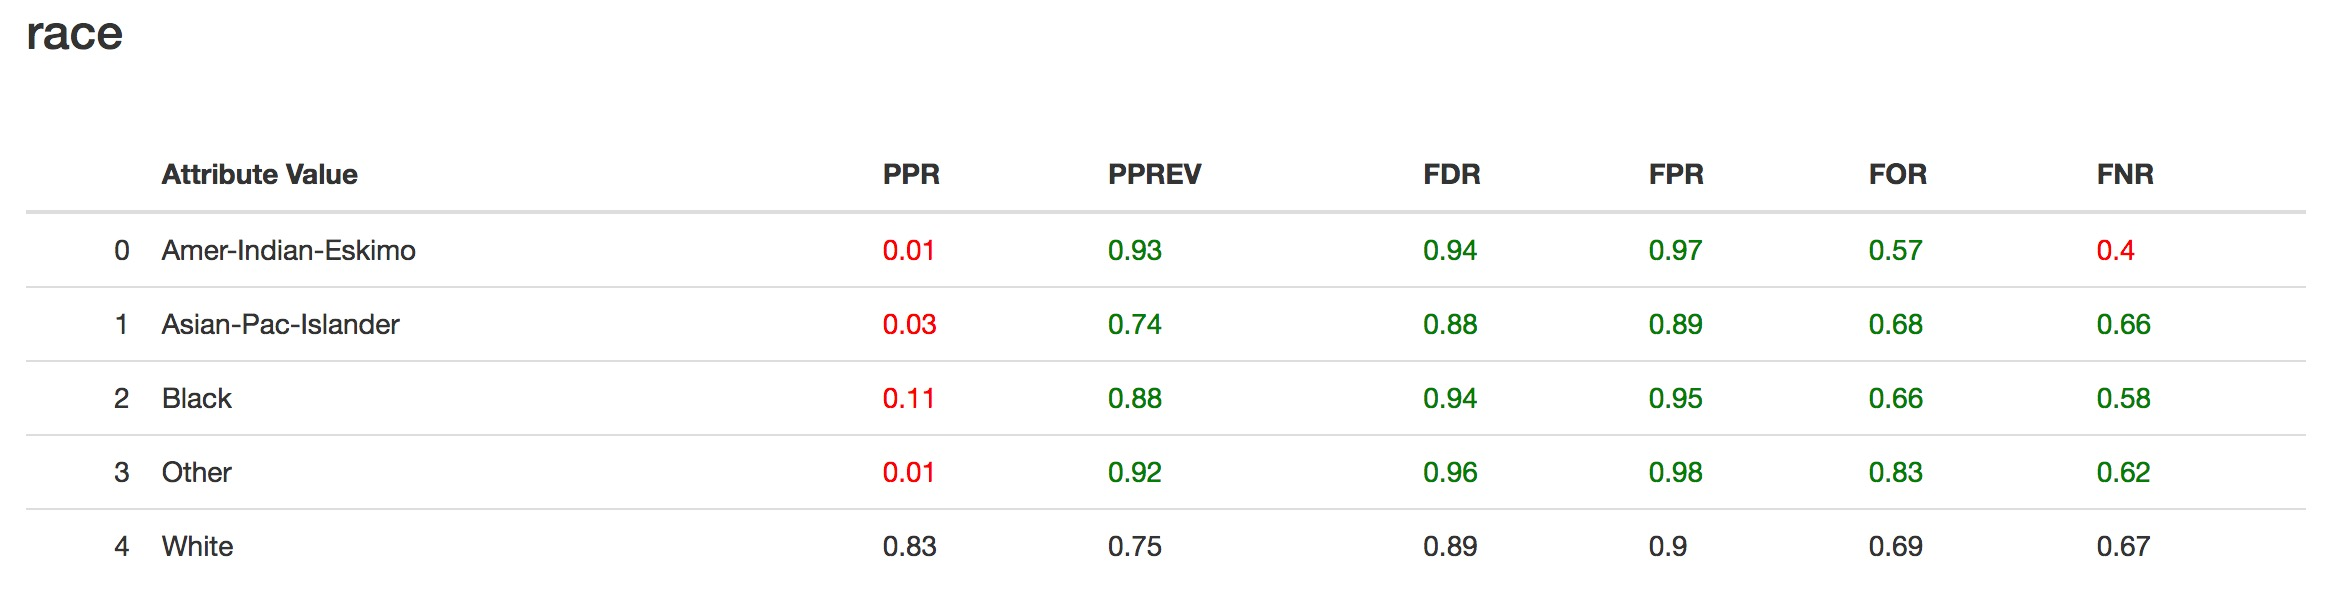
\includegraphics[width=17.5cm]{group_adult_aq.jpg}
	\caption{Tabla con las principales métricas de grupo para el atributo \textit{race}.}
    \label{fig:ejaq1}
\end{figure}

\subsubsection{Métricas de sesgo}

Mide la disparidad entre un grupo y el grupo de referencia. La disparidad se calcula a partir de la siguiente fórmula: $$DisparityMeasure_{ProtectedGroup}=\ddfrac{GroupMetric_{ProtectedGroup}}{GroupMetric_{ReferenceGroup}}$$ Donde $GroupMetric$ hace referencia a una métrica de grupo del Cuadro \ref{tab:groupmetricaq}. Es evidente que la disparidad de cualquier medida sobre el grupo de referencia siempre será 1. Si queremos calcular por ejemplo la disparidad del ratio de falsos negativos ($FNR$) sobre el grupo de raza negra, se calculará de la siguiente forma: $$FNR_{Black}=\ddfrac{FNR_{Black}}{FNR_{White}}=\ddfrac{0.58}{0.67}=0.86$$

Completando la tabla para todas las métricas de grupo obtenemos el siguiente resultado:

\begin{figure}[h]
	\centering
	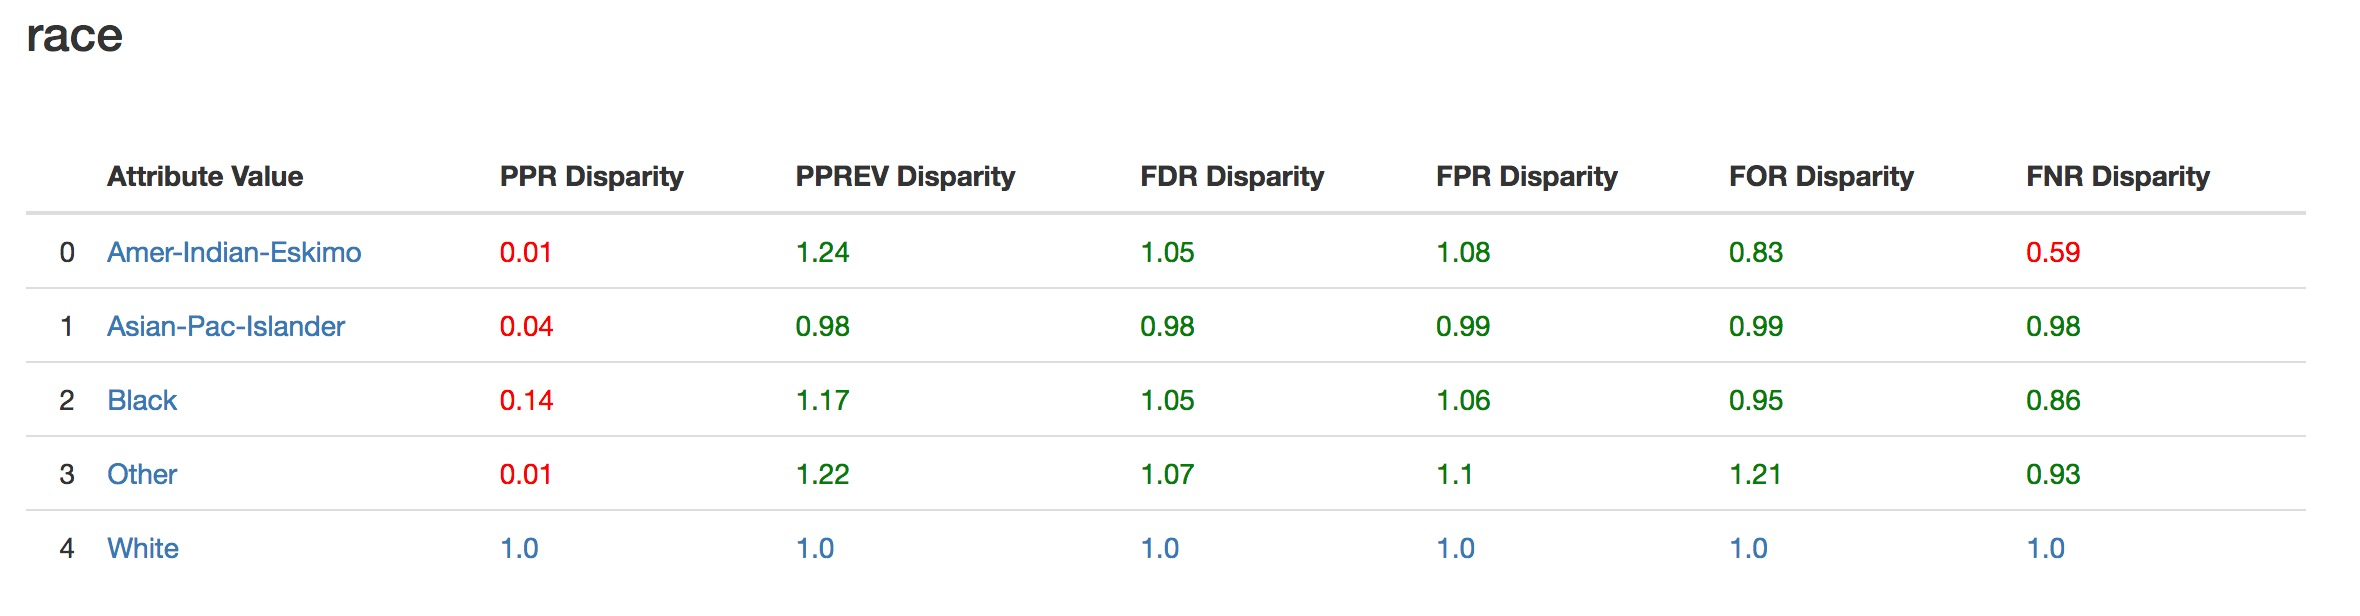
\includegraphics[width=17.5cm]{disparity_adult_aq.jpg}
	\caption{Tabla con las métricas de sesgo para el atributo \textit{race}.}
    \label{fig:ejaq2}
\end{figure}

\begin{remark}
De forma predeterminada, Aequitas usa el grupo mayoritario dentro de cada atributo como grupo de referencia.
\end{remark}

\subsubsection{Medidas de equidad}

La equidad siempre se define en relación con un grupo de referencia. Podemos ver que el cálculo de la equidad, depende de la métrica de sesgo. En la evaluación del criterio de equidad, un grupo cumple con la paridad si $$(1-\varepsilon)\leq \text{DisparityMeasure}_{\text{group}_i} \leq \ddfrac{1}{(1-\varepsilon)}$$ donde $\varepsilon$ es el umbral de equidad definido.

Tomando $\varepsilon=0.2$ cualquier métrica de sesgo se considerará justa en el intervalo $$\left[1-0.2,\ddfrac{1}{1-0,2}\right]=[0.8,1.25]$$

En el informe de resultados final que devuelve Aequitas si todas las métricas de equidad contienen el flag \textit{fair}, se evaluará el modelo actual como justo. De lo contrario, lo considerará injusto y enumerará los grupos afectados injustamente según los criterios de equidad dados.

\begin{figure}[h]
	\centering
	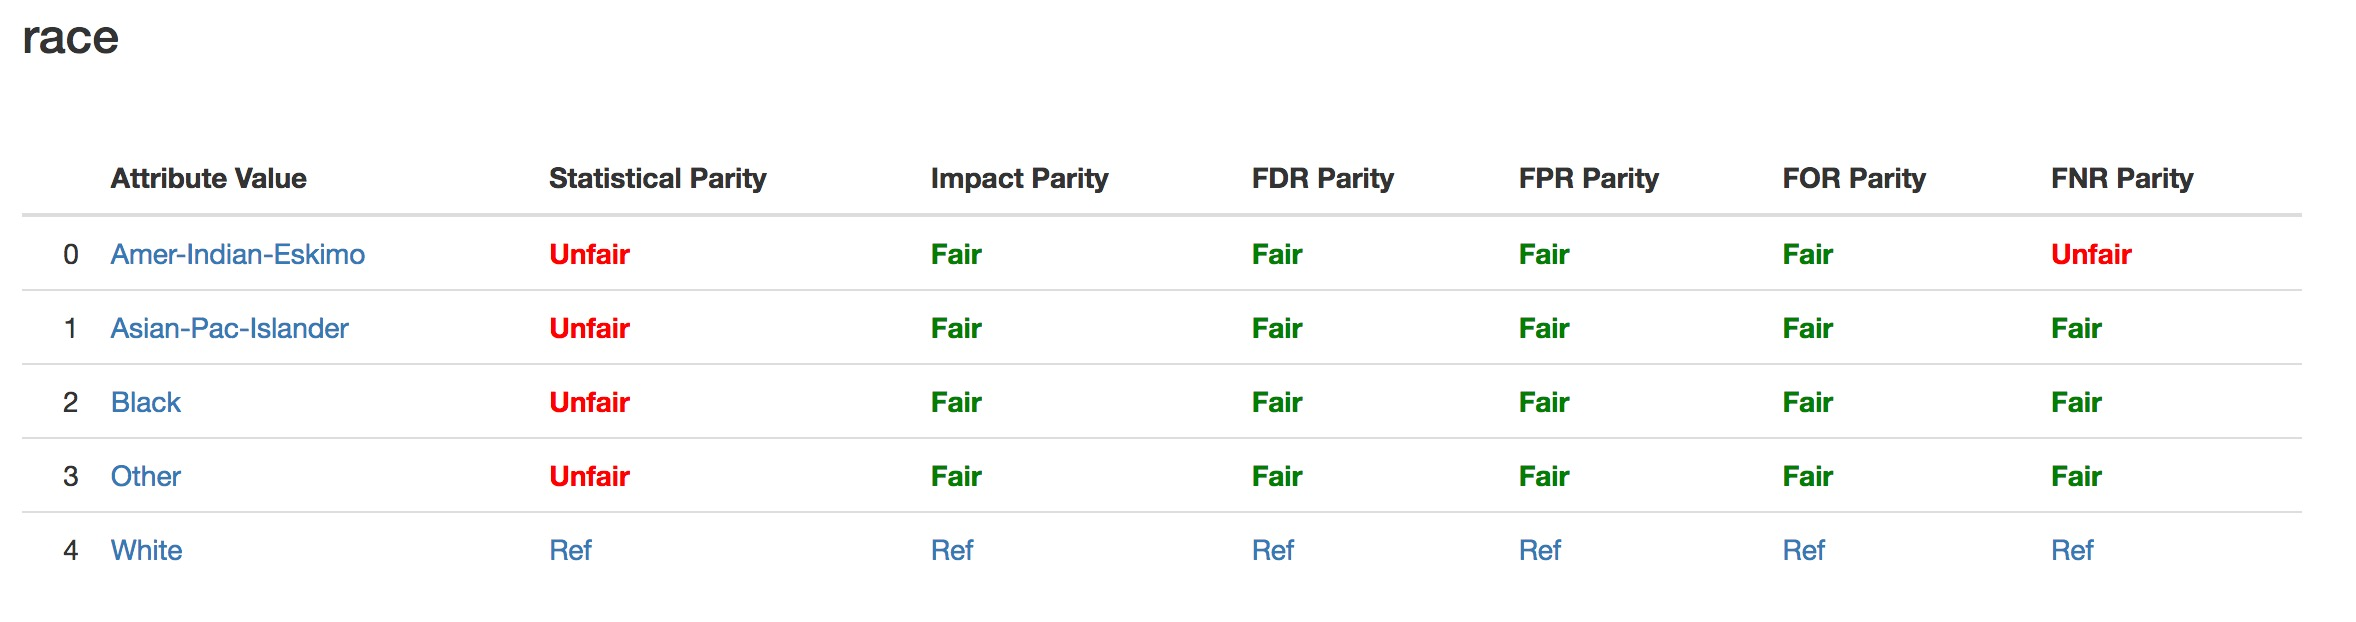
\includegraphics[width=17.5cm]{fairness_adult_output.jpg}
	\caption{Tabla de medidas de equidad aplicado el umbral.}
    \label{fig:medequmbral}
\end{figure}

\begin{figure}[h]
	\centering
	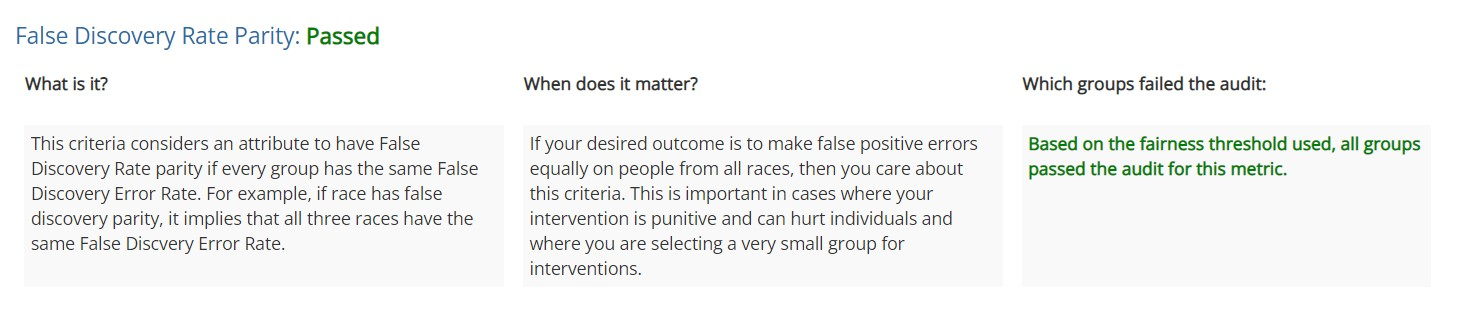
\includegraphics[width=17.5cm]{fairness_output_aq.jpg}
	\caption{Resultado del modelo injusto.}
    \label{fig:ejunfairaq}
\end{figure}

En la Figura \ref{fig:ejunfairaq} podemos ver que el modelo no cumple con los criterios de Paridad Falsa Negativa (\textit{False Negative Parity}) y de Igual Paridad (\textit{Equal Parity}).

Podemos ver que los conceptos de equidad que utiliza Aequitas son los siguientes:

\begin{itemize}
    \item Equal Parity.
    \item Proportional Parity.
    \item False Positive Parity.
    \item False Negative Parity.
\end{itemize}

\textcolor{red}{La versión actual es un esquema de lo que se intentará mostrar con imágenes sacadas de la web que deben cambiarse. Idea probar en Aequitas con las medidas existentes el mismo dataset que usaré con contrafactual, si no se puede, usar COMPAS.}